% This is text associated with the open textbook "Open Electromagnetics"
% See immediately below for author, date
% This work is licensed under the Creative Commons Attribution-ShareAlike 4.0 International License. (CC BY-SA 4.0) 
% To view a copy of the license, visit http://creativecommons.org/licenses/by-sa/4.0/

%ORB TITLE Curl
%ORB AUTHOR 0        # S.W. Ellingson, Virginia Tech (ellingson@vt.edu)
%ORB DATE 20180803   # yyyymmdd
%ORB ABSTRACT Curl

\label{m0048_Curl} % <-- Must match name of this file and module directory name.  Don't mess with this!
\index{curl|(}

\index{circulation|(}

Curl is an operation, which when applied to a vector field, quantifies the \emph{circulation} of that field.
The concept of circulation has several applications in electromagnetics.
Two of these applications correspond to directly to Maxwell's Equations:
%
\begin{itemize}
\item The circulation of an electric field is proportional to the rate of change of the magnetic field.  This is a statement of the \emph{Maxwell-Faraday Equation} 
\index{Maxwell-Faraday equation}
(Section~\ref{m0050_Maxwell-Faraday_Equation}), which includes as a special case \emph{Kirchoff's Voltage Law for electrostatics} 
\index{Kirchoff's voltage law!electrostatics}
(Section~\ref{m0152_KVL_Electrostatics_Integral-to-Differential}).
\item The circulation of a magnetic field is proportional to the source current and the rate of change of the electric field.  This is a statement of \emph{Ampere's Law} 
\index{Ampere's law!magnetostatics}
(Sections~\ref{m0118_Amperes_Law_Magnetostatics_Integral-to-Differential} and \ref{m0053_Displacement_Current_Amperes_Law})
\end{itemize}
%
Thus, we are motivated to formally define circulation and then to figure out how to most conveniently apply the concept in mathematical analysis.  The result is the \emph{curl} operator.   

So, we begin with the concept of circulation:
%
%ORB HIGHLIGHT
\begin{mdframed}[backgroundcolor=yellow!20,nobreak=true] 
``Circulation'' is the integral of a vector field over a closed path.
\end{mdframed}
%
Specifically, the circulation of the vector field ${\bf A}({\bf r})$ over the closed path ${\mathcal C}$ is
%
\begin{equation}
\oint_{\mathcal C} {\bf A}\cdot d{\bf l}
\end{equation}
%
The circulation of a uniform vector field is zero for any valid path. 
For example, the circulation of ${\bf A}=\hat{\bf x}A_0$ is zero because non-zero contributions at each point on ${\mathcal C}$ cancel out when summed over the closed path.
On the other hand, the circulation of ${\bf A}=\hat{\bf \phi}A_0$ over a circular path of constant $\rho$ and $z$ is a non-zero constant, since the non-zero contributions to the integral at each point on the curve are equal and accumulate when summed over the path. 

%ORB EXAMPLE
~\\ \begin{example} 
\begin{mdframed}[backgroundcolor=brown!20,linecolor=brown!20]\raggedright
Circulation of the magnetic field intensity surrounding a line current. 
\\~\\
Consider a current $I$ (units of A) flowing along the $z$ axis in the $+z$ direction, as shown in Figure~\ref{m0048_fBiotSavartExample}.
%
It is known that this current gives rise to a magnetic field intensity ${\bf H} = \hat{\bf \phi}H_0/\rho$, where $H_0$ is a constant having units of A since the units of ${\bf H}$ are A/m. (Feel free to consult Section~\ref{m0119_Magnetic_Field_of_a_Long_Wire} for the details; however, no additional information is needed to follow the example being presented here.)
The circulation of ${\bf H}$ along any circular path of radius $a$ in a plane of constant $z$ is therefore
%
\begin{equation}
\oint_{\mathcal C} {\bf H}\cdot d{\bf l} 
= \int_{\phi=0}^{2\pi} \left( \hat{\bf \phi}\frac{H_0}{a} \right) \cdot \left( \hat{\bf \phi}~a~d\phi \right) 
= 2\pi H_0
\nonumber
\end{equation}
%
Note that the circulation of ${\bf H}$ in this case has two remarkable features: 
(1) It is independent of the radius of the path of integration; and 
(2) it has units of A, which suggests a current. 
In fact, it turns out that the circulation of ${\bf H}$ in this case is \emph{equal} to the enclosed source current $I$.
Furthermore, it turns out that the circulation of ${\bf H}$ along \emph{any} path enclosing the source current is equal to the source current!
These findings are consequences of \emph{Ampere's Law}, as noted above.
\end{mdframed}
%
\begin{figure}
\begin{center}
\pdftooltip{{  % note double braces
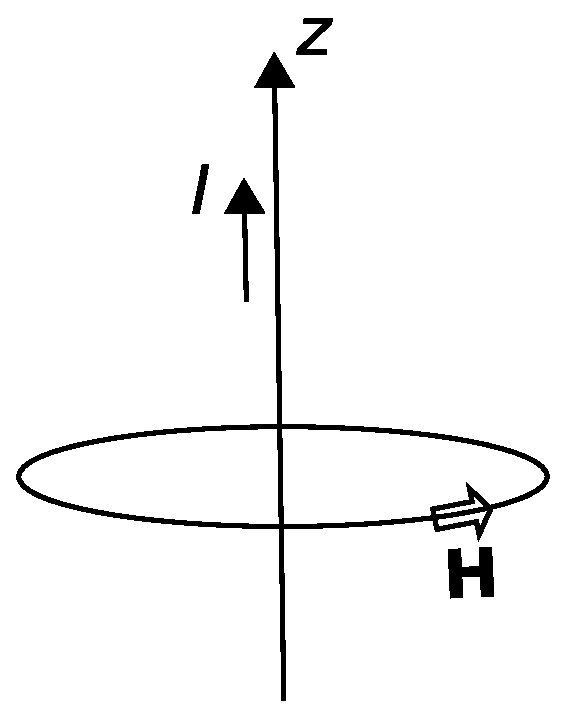
\includegraphics[width=1.5in]{modules/m0048_fBiotSavartExample.eps}
% https://commons.wikimedia.org/wiki/File:Biot_Savart_Example.svg
}}{A z-axis extends upward, with an arrow pointing in the positive z direction to indicate current direction. A circle around the z-axis shows an arrow in a counterclockwise direction labeled H to indicate magnetic field intensity.}
\end{center} 
\centerline{\scriptsize 
\copyright~\hyperref[m0048_fBiotSavartExample_Credit]{K.\ Kikkeri} 
\href{https://creativecommons.org/licenses/by-sa/4.0/}{CC BY~SA 4.0} 
} 
\caption{
\label{m0048_fBiotSavartExample}
Magnetic field intensity due to a current flowing along the $z$ axis.
}
\end{figure}
\end{example}

\index{circulation|)}

Curl is, in part, an answer to the question of what the circulation \emph{at a point in space} is.
In other words, what is the circulation as ${\mathcal C}$ shrinks to it's smallest possible size.  
The answer in one sense is zero, since the arclength of ${\mathcal C}$ is zero in this limit -- there is nothing to integrate over.
However, if we ask instead what is the circulation \emph{per unit area} in the limit, then the result should be the non-trivial value of interest. 
To express this mathematically, we constrain ${\mathcal C}$ to lie in a plane, and define ${\mathcal S}$ to be the open surface bounded by ${\mathcal C}$ in this case.
Then, we define the scalar part of the curl of ${\bf A}$ to be:
%
\begin{equation}
\lim_{\Delta s \to 0} \frac{\oint_{\mathcal C} {\bf A}\cdot d{\bf l}}{\Delta s}
\end{equation}
%
where $\Delta s$ is the area of ${\mathcal S}$, and (important!) we require ${\mathcal C}$ and ${\mathcal S}$ to lie in the plane that maximizes the above result. 

Because ${\mathcal S}$ and it's boundary ${\mathcal C}$ lie in a plane, it is possible to assign a direction to the result.
The chosen direction is the normal $\hat{\bf n}$ to the plane in which ${\mathcal C}$ and ${\mathcal S}$ lie.
Because there are two normals at each point on a plane, we specify the one that satisfies the \emph{right hand rule}.
This rule, applied to the curl, states that the correct normal is the one which points through the plane in the same direction as the fingers of the right hand when the thumb of your right hand is aligned along ${\mathcal C}$ in the direction of integration.
Why is this the correct orientation of $\hat{\bf n}$?  
See Section~\ref{m0051_Stokes_Theorem} for the answer to that question.
For the purposes of this section, it suffices to consider this to be simply an arbitrary sign convention.
  
Now with the normal vector $\hat{\bf n}$ unambiguously defined, we can now formally define the curl operation as follows:
\index{curl!definition}
%
\begin{equation}
\mbox{curl}~{\bf A} \triangleq \lim_{\Delta s \to 0} \frac{\hat{\bf n}\oint_{\mathcal C} {\bf A}\cdot d{\bf l}}{\Delta s}
\label{m0048_eCurlDef}
\end{equation}
%
where, once again, $\Delta s$ is the area of ${\mathcal S}$, and we select ${\mathcal S}$ to lie in the plane that maximizes the magnitude of the above result.  Summarizing:

%ORB HIGHLIGHT
\begin{mdframed}[backgroundcolor=yellow!20,nobreak=true] 
The curl operator quantifies the circulation of a vector field at a point.
\end{mdframed}

%ORB HIGHLIGHT
\begin{mdframed}[backgroundcolor=yellow!20,nobreak=true] 
The magnitude of the curl of a vector field is the circulation, per unit area, at a point and such that the closed path of integration shrinks to enclose zero area while being constrained to lie in the plane that maximizes the magnitude of the result.
\end{mdframed}

%ORB HIGHLIGHT
\begin{mdframed}[backgroundcolor=yellow!20,nobreak=true] 
The direction of the curl is determined by the right-hand rule applied to the associated path of integration.
\end{mdframed}

Curl is a very important operator in electromagnetic analysis.
However, the definition (Equation~\ref{m0048_eCurlDef}) is usually quite difficult to apply.
Remarkably, however, it turns out that the curl operation can be defined in terms of the $\nabla$ operator; that is, the same $\nabla$ operator associated with the gradient, divergence, and Laplacian operators.  Here is that definition:
%
\begin{equation}
\mbox{curl}~{\bf A} \triangleq \nabla \times {\bf A}
\end{equation}
%
For example:
In Cartesian coordinates,
%
\begin{equation}
\nabla \triangleq \hat{\bf x}\frac{\partial}{\partial x} + \hat{\bf y}\frac{\partial}{\partial y} + \hat{\bf z}\frac{\partial}{\partial z} 
\end{equation}
%
and
%
\begin{equation}
{\bf A} = \hat{\bf x}A_x + \hat{\bf y}A_y + \hat{\bf z}A_z 
\end{equation}
%
so curl can be calculated as follows:
%
\begin{equation}
\nabla\times{\bf A} =
\begin{vmatrix}
\hat{\bf x} & \hat{\bf y} & \hat{\bf z} \\
\frac{\partial}{\partial x} & \frac{\partial}{\partial y} & \frac{\partial}{\partial z} \\
A_x & A_y & A_z 
\end{vmatrix}
\end{equation}
%
or, evaluating the determinant:
%   
\begin{equation}
\begin{split}
\nabla \times {\bf A} &= \hat{\bf x}\left( \frac{\partial A_z}{\partial y} - \frac{\partial A_y}{\partial z} \right) \\
                      &~~ +\hat{\bf y}\left( \frac{\partial A_x}{\partial z} - \frac{\partial A_z}{\partial x} \right) \\
                      &~~ +\hat{\bf z}\left( \frac{\partial A_y}{\partial x} - \frac{\partial A_x}{\partial y} \right) 
\end{split}
\end{equation}
%
Expressions for curl in each of the three major coordinate systems is provided in Appendix~\ref{m0139_Vector_Operators}. 

It is useful to know is that curl, like $\nabla$ itself, is a linear operator; that is, for any constant scalars $a$ and $b$ and vector fields ${\bf A}$ and ${\bf B}$:
%
\begin{equation}
\nabla \times \left( a{\bf A} + b{\bf B} \right) = a \nabla \times {\bf A} + b \nabla \times {\bf B}
\end{equation}

%%%%%%%%%%%%%%%%%%%%%%%%%%%%%%%%%%%%

{\bf Additional Reading:}
\begin{itemize}
\item ``\href{https://en.wikipedia.org/wiki/Curl_(mathematics)}{Curl (mathematics)}'' on Wikipedia.
\end{itemize}

\index{curl|)}


